\documentclass[spanish]{textolivre}

% metadata
\journalname{Texto Livre}
\thevolume{17}
%\thenumber{1} % old template
\theyear{2024}
\receiveddate{\DTMdisplaydate{2024}{3}{19}{-1}}
\accepteddate{\DTMdisplaydate{2024}{6}{23}{-1}}
\publisheddate{\today}
\corrauthor{Lorena Berríos Barra}
\articledoi{10.1590/1983-3652.2024.51684}
%\articleid{NNNN} % if the article ID is not the last 5 numbers of its DOI, provide it using \articleid{} commmand 
% list of available sesscions in the journal: articles, dossier, reports, essays, reviews, interviews, editorial
\articlesessionname{articles}
\runningauthor{Berríos Barra}
%\editorname{Leonardo Araújo} % old template
\sectioneditorname{Hugo Heredia Ponce}
\layouteditorname{João Mesquita}

\title{Prácticas de literacidad digital y mediación de la literatura en el profesorado en formación: experiencias a través de portafolios reflexivos digitales}
\othertitle{Práticas de letramento digital e mediação literária em professores em formação: experiências através de portfólios reflexivos digitais}
\othertitle{Digital literacy practices in pre-service teaching: experiences of mediating literature through reflective digital portfolios}

\author[1]{Lorena Berríos Barra~\orcid{0000-0003-3698-1712}\thanks{Email: \href{mailto:lorena.berrios@uchile.cl}{lorena.berrios@uchile.cl}}}
\affil[1]{Universidad de Chile, Departamento de Estudios Pedagógicos de la Facultad de Filosofía y Humanidades, Santiago, Ñuñoa, Chile.}


\addbibresource{article.bib}
%\usepackage{longtable}

\begin{document}
\maketitle

\begin{polyabstract}
\begin{abstract}
La lectura, después de la pandemia de COVID-19, requiere de perspectivas
diferentes para su mediación. Este artículo presenta una experiencia de
mediación, por medio de la valoración de seis portafolios reflexivos
digitales de futuros docentes chilenos de la Universidad de Chile
desarrollados durante el año académico 2022 y 2023. La valoración de los
portafolios se realizó considerando marcos sobre literacidades
digitales. El objetivo de la creación de portafolios fue desplegar las
literacidades digitales de los profesores en formación y presentar
experiencias de mediación de la literatura que integran la pedagogía de
las multiliteracidades. Las literacidades digitales presentes en los
portafolios se manifiestan a través del lenguaje de internet como el uso
de memes, la gamificación e itinerarios que reflejan un diseño
multimodal. Las plataformas digitales utilizadas son aquellas propuestas
para el ámbito educativo. Las experiencias de mediación de la
literatura, expuestas en estos portafolios, incorporan parte de las
literacidades digitales de futuros docentes, ya que la lectura está
mediada desde las manifestaciones culturales y digitales conocidas por
sus estudiantes y no desde los textos literarios en sí. Como conclusión,
se señala la necesidad de generar instancias formativas que permitan
concientizar a futuros docentes sobre sus literacidades digitales para
que puedan ser integradas en procesos de mediación que permitan la
agencia del estudiantado y, de este modo, hacer frente a los desafíos
que presenta la lectura literaria en la escuela.

\keywords{Alfabetización digital \sep Formación preparatoria de docentes \sep Enseñanza de la literatura \sep Plataforma digital}
\end{abstract}

\begin{portuguese}
\begin{abstract}
A leitura, após a pandemia do COVID-19, requer diferentes perspectivas
para sua mediação. Este artigo apresenta uma experiência de mediação,
por meio da avaliação de seis portfólios reflexivos digitais de futuros
professores chilenos da Universidade do Chile, desenvolvidos durante o
ano acadêmico de 2022 e 2023. A avaliação dos portfólios foi realizada
considerando marcos sobre letramentos digitais. O objetivo da criação
dos portfólios foi mostrar os letramentos digitais dos professores em
formação e apresentar experiências de mediação da literatura que
integram a pedagogia dos multiletramentos. Os letramentos digitais
presentes nos portfólios manifestam-se através da linguagem da Internet,
como a utilização de memes, a gamificação e itinerários que refletem um
\textit{design} multimodal. As plataformas digitais utilizadas são aquelas
propostas para a esfera educacional. As experiências de mediação da
literatura, apresentadas nesses portfólios, incorporam parte dos
letramentos digitais dos futuros professores, uma vez que a leitura é
mediada a partir das manifestações culturais e digitais conhecidas por
seus alunos e não a partir dos textos literários em si. Em conclusão,
apontamos a necessidade de gerar instâncias de formação que permitam aos
futuros professores tomarem consciência de seus letramentos digitais para
que possam ser integrados em processos de mediação que permitam a
agência dos alunos e, dessa forma, enfrentar os desafios apresentados
pela leitura literária na escola.

\keywords{Letramento digital \sep Formação de professores preparatórios \sep Ensino da literatura \sep Plataforma digital}
\end{abstract}
\end{portuguese}

\begin{english}
\begin{abstract}
Reading after the COVID-19 pandemic requires different perspectives for
its mediation. This article presents an experience of mediation through
the assessment of six digital reflective portfolios from future Chilean
teachers at a University of Chile. This potfolios were developed during
the academic years 2022 and 2023. The assessment of the portfolios was
conducted considering frameworks on digital literacies. The objective of
creating portfolios was to showcase the digital literacies of
pre-service teachers and present experiences of literature mediation
that integrate the pedagogy of multiliteracies. The digital literacies
present in portfolios are expressed through internet language, such as
the use of memes, gamification, and itineraries thar reflect a
multimodal design. The digital platforms used are those recommended for
educational field. The experiences of literature mediation, as showcased
in this portfolios, incorporate aspects of the digital literacies of
future educators. Reading is mediated through cultural and digital
expressions known to their students rather than solely through literary
texts. In conclusion, there is a need to create training opportunities
that raise awareness among future teachers about their integration into
mediation processes that empower student. This approach aims to address
the challenges posed by literary reading in schools.

\keywords{Digital literacy \sep Preservice teacher \sep Literature
education \sep Digital platforms}
\end{abstract}
\end{english}
\end{polyabstract}

\section{Introducción}\label{sec-Introducción}

La evolución de la inteligencia artificial (IA) ha marcado un hito
significativo en la actualidad sofocada por infodemia e infoxicación.
Esta transformación tecnológica, inicialmente concebida por John
McCarthy en 1956, ha avanzado significativamente, incorporando
aplicaciones de aprendizaje automático y procesamiento del lenguaje
natural (NLP) en herramientas educativas \cite{Sadiku2021}. No obstante, el gran salto se dio con la presentación de
ChatGPT en 2020, y con mejor respuesta a principios del 2023, siendo la
IA Generativa (IAGen) otra forma de entender a la IA; la IAGen crea
contenido original a partir de datos existentes mediante algoritmos y
redes neuronales avanzadas \cite{Feuerriegel2024}.

En el campo de la educación, los modelos de lenguaje grandes (LLM,
\emph{Large Language Model}), como ChatGPT \cite{OpenAI2023}, ha generado
diversos debates públicos y digitales como el de la opinión emitida por
el lingüista {\textcite{Chomsky2023}}, donde califica a ChatGPT como una forma de plagio de alta
tecnología, pudiendo socavar la educación al motivar a los estudiantes
en la búsqueda de atajos para la entrega de trabajos, como los ya
clásicos ensayos o resolución a preguntas cerradas, como en un
cuestionario de reforzamiento, por ejemplo. Ante este tipo de
reflexiones, han surgido otras como la de \textcite{Yell2023}, un
profesor retirado de la Universidad de Wisconsin, argumentan sobre que,
si se utiliza de forma adecuada, ChatGPT puede ser un recurso valioso
para fomentar el aprendizaje basado en la búsqueda e investigación,
permitiendo promover el pensamiento crítico. Aunque es indiscutible que
este tipo de tecnología es capaz de crear contenido nuevo en formato de
texto, imágenes o audio, permitiendo hasta asistir en tareas de
conocimiento y necesidades cotidianas \cite{Feuerriegel2024}.

La aplicación de ChatGPT en la educación se ve reflejada en el análisis
de \textcite{Dimitriadou2023}, quienes abordan la integración de la
IA en las aulas inteligentes y los desafíos éticos asociados, así como
en el estudio de \textcite{Tlili2023} abordando el uso de
\emph{chatbots}, que examinan la aplicación de ChatGPT en la elaboración
de ejercicios en forma de cuestionarios. Estos enfoques resaltan el
equilibrio necesario entre las capacidades de la IA y la intervención
humana para garantizar la relevancia, la exactitud y la equidad en la
educación.

Recientes investigaciones, como las de \textcite{Nasution2023} y \textcite{Ruiz2023},
han explorado el uso de ChatGPT 4.0 en la generación de ítems de examen,
destacando no solo su capacidad para crear preguntas de elección
múltiple relevantes y coherentes, sino también abordando desafíos como
irregularidades y redundancias en interacciones más prolongadas. Estos
estudios subrayan la importancia de la especificidad y sistematización
en los prompts para generar exámenes eficientes y precisos,
capitalizando las fortalezas de la IA para la educación \cite{Nasution2023, Ruiz2023}.

La investigación de \textcite{Nasution2023} se enfocó en la validez y
confiabilidad de las preguntas generadas por IA, un tema que ha
suscitado tanto interés como preocupación en la comunidad educativa. Con
una muestra de 272 estudiantes, Nasution emprendió la tarea de evaluar
una serie de preguntas creadas por ChatGPT, obteniendo resultados que
son tanto prometedores como reveladores. De las 21 preguntas generadas
por la IA, 20 resultaron ser válidas, lo que indica una alta tasa de
éxito. Este hallazgo es significativo, ya que subraya la capacidad de la
IA para producir contenido educativo que no solo es relevante, sino
también de calidad.

No obstante, también hay investigaciones en torno al uso de Machine
Learning (ML) como el de \textcite{Rauber2024} quienes desarrollaron un
modelo automatizado para medir el aprendizaje de conceptos y prácticas
de clasificación de imágenes mediante redes neuronales. Se basó en datos
de 240 estudiantes de secundaria y bachillerato, concluyendo que la
evaluación es confiable y válida. Además, destacaron la efectividad del
modelo resaltando la importancia de incluir ML en la educación escolar y
la capacidad del modelo para asistir en el proceso de evaluación,
facilitando la carga de trabajo de los docentes.

A medida que la tecnología de IA continúa evolucionando, con avances
significativos en las versiones más recientes de ChatGPT, se presenta
una oportunidad única para mejorar y sistematizar el proceso de creación
de exámenes. Las investigaciones de \textcite{Nasution2023,Ruiz2023} se
alinean con esta visión, proponiendo un enfoque metodológico que combina
la exploración y descripción detallada de las capacidades de ChatGPT 4.0
en la generación de ítems de examen, proporcionando así una perspectiva
integral de su aplicabilidad y eficacia en el ámbito educativo. No
obstante, todavía hacen falta estudios que comparen el comportamiento de
la IAGen y si los seres humanos somos capaces de detectar esas
diferencias, o bien, podrían ayudar a reducir la carga de los docentes e
instituciones al momento de crear exámenes de alto impacto; como los del
ingreso a la universidad.

Ante todos estos acontecimientos, y retomando estos modelos de lenguaje
que podrían ayudarnos a evaluar nuestra propia forma de comunicar, el
objetivo principal de esta investigación fue explorar y comparar la
eficacia de la IAGen, representada por ChatGPT 4.0, y los diseñadores
humanos en el desarrollo de ítems para el Examen de Ingreso a la
Educación Superior (ExIES), en el área de Lengua Escrita, a través del
método de juicio de expertos. Lo anterior, con el fin determinar la
calidad, relevancia y alineación de los ítems generados por ambas
fuentes (IA y humanos) con los estándares establecidos para la
evaluación educativa, centrándose en aspectos como claridad,
neutralidad, concisión, alineación curricular y adecuación de formato y
contenido.
\section{Prácticas de literacidad digital en la mediación de la
	literatura}\label{prácticasdeliteracidad}
	
	En la formación inicial docente, la mediación de la literatura a través
	de tecnologías digitales ha sido abordada en el último tiempo como una
	preocupación ante la forma de concebir la lectura por parte de las
	nuevas generaciones \cite{contrereasbarcelo2023,gonzalez_2016,rovira-collado2021}. Los estudios han señalado,
	especialmente, la relación de futuros docentes con internet, las redes
	sociales y sus posibilidades para la enseñanza de la literatura. Dichos
	estudios proponen un enfoque desde la multimodalidad, las
	multiliteracidades y la lectura en formatos digitales, como una forma de
	acoger a los nuevos lectores que definen su relación con la lectura a
	través de los dispositivos digitales, las redes sociales e internet.
	
	La discusión sobre el nuevo lector \cite{cerrillo2005,lluch_2010_new,montesa_et_al_2010}, ha advertido de la interacción de los
	niños y adolescentes con los formatos digitales y de la posibilidad de
	acceder a otra experiencia de lectura, cuyos fines son más prácticos
	\cite{oecd_2019b}. La pandemia pudo haber intensificado este aspecto, ya que
	la lectura que realizan los estudiantes se da, mayormente, en formatos
	digitales. Estudios señalan que los jóvenes realizan una lectura que se
	centra en la obtención de información, comunicación y socialización
	\cite{Valdivia_Brossi_Cabalin_Pinto_2019}, pero que no necesariamente desarrolla el
	pensamiento crítico y la capacidad de agencia \cite{cabero-almenara_valencia-ortiz_llorente-cejudo_palacios-rodríguez_2023}.

En este sentido, se ha señalado la necesidad de desarrollar un enfoque diferente para la lectura literaria a través de soportes digitales \cite{cordongarcias2015,garciaroca2016practicas}, ya que el estudiante sería un lector implícito \cite{turreonpenelas2014}. No obstante, uno de los principales problemas para llevar a cabo dicha lectura dentro del aula es la escasez de dispositivos interactivos digitales en las escuelas \cite{ramadaprietoturrion2019}, que dificultaría desarrollar estrategias de mediación diferentes.
	
Como una forma de atender a los problemas en torno a la mediación de la
literatura y la formación de lectores, en el último tiempo se ha
indagado en las trayectorias lectoras de futuros profesores, en que se
ha señalado que los docentes son las figuras más relevantes en la
mediación de la literatura en el aula \cite{contrerasbarcelo2021}. Dentro
de esta idea, también se ha indagado en futuros docentes como lectores
en medios digitales y creadores dentro de escenarios transmedia, donde
han revelado la necesidad de ser formados en interpretación, reflexión y
evaluación de contenidos transmedia en un contexto formal \cite{contrereasbarcelo2023}, que da cuenta del cambio de paradigma en
torno a la lectura literaria y la formación de lectores.
	
Considerando los aspectos señalados anteriormente, cabe preguntarse por
los cambios que requiere la enseñanza de la literatura y de cuál es el
lugar de las literacidades digitales de profesores en formación dentro
de la interacción didáctica. Uno de los aspectos que han sido estudiados
en torno a dicha inquietud, tiene relación con el desarrollo de la
competencia digital pedagógica en profesores en formación y sus
limitaciones, que podrían dificultar el desarrollo de estrategias que
puedan mediar textos literarios a través del uso de tecnología digital.
Diversos autores han señalado la necesidad de formar pedagógicamente en
el uso de las TIC a los futuros docentes \cite{ayala2015,sandoval-rubilar_alveal_fuentes_2017,Silva_Morales_Lázaro-Cantabrana_Gisbert_Miranda_Rivoir_Onetto_2019},
ya que, en general, existe un desconocimiento del uso pedagógico de las
herramientas digitales.
	
En este sentido, es necesario que las tecnologías digitales sean
integradas de manera pedagógica en el desarrollo de estrategias y en la
mediación de textos literarios, considerando lo que se ha señalado sobre
los nuevos lectores y las prácticas digitales de los adolescentes, que
inciden en el tipo de lectura que realizan. No obstante, dentro de las
dificultades para la enseñanza de la literatura y su mediación, están
las concepciones que tiene el profesorado sobre la literatura \cite{barra2022} y las estrategias que se requieren para enseñarla
en soportes digitales, que son diferentes a la lectura en soporte
analógico \cite{ryan_2004}.

Una manera de abordar estos asuntos puede ser a través de la integración
de las literacidades digitales de docentes en formación en las
estrategias para mediar la literatura. Cabe precisar al respecto, que la
definición de las literacidades digitales posee límites imprecisos
\cite{manghi_haquin_2016,villar_onrubia_morini_marin_nascimbeni_2022},
no obstante, para la valoración de los portafolios, se ha considerado
desde una perspectiva sociocultural y con prácticas que van más allá de
la lectura y escritura \cite{villar_onrubia_morini_marin_nascimbeni_2022}. Dichas
prácticas se desarrollan dentro de un marco que participa tanto de lo
cultural como de lo histórico e institucional \cite{gee2015} y que
interactúan con formas post-tipográficas de textos y su producción
\cite{lankshear_knobel_2008}.

Las literacidades digitales, dentro de la experiencia desarrollada, se
han acotado a lo que proponen \textcite[p. 9]{gillen_barton_2010}, que las definen como
``prácticas en constante cambio, a través de las cuales las personas
crean significados rastreables utilizando tecnologías digitales'' y, por
tanto, ``implican una atención cuidadosa y sensible a lo que las
personas hacen con los textos ``.

Dentro del desarrollo de los portafolios se dio énfasis a la interacción
de los futuros docentes con las tecnologías digitales y que, en dicha
interacción, se reflejaran sus recursos e ideología, para trascender,
así, el uso técnico de las TIC \cite{dowdall2021digital}.

En la formación inicial y continua del profesorado, se ha dado
importancia a la introducción de las prácticas de literacidad en la
enseñanza, que están fuertemente ligadas al uso de tecnologías digitales
\cite{thibaut_2020}, y también, al desarrollo de las multiliteracidades para
la mediación de la literatura \cite{godoy2023,cabrerocafort2021}, que
se ha visto como una posibilidad tangible y necesaria. En Chile es
relevante su introducción en el aula, debido a la presencia que tiene la
multimodalidad dentro del currículo nacional \cite{meneses_literacidad_2023}.

En relación con lo anterior, hay experiencias que han abordado la
mediación de la literatura a través de la noción de diseño de las
multiliteracidades, la cual se entiende dentro de la gramática de la
multimodalidad. La idea de diseño disponible (recursos), de diseñar
(producir significado) y de rediseño (diseños disponibles nuevos)
\cite{kalantzis_cope_new_learning}, han posibilitado a los estudiantes profundizar
la lectura y reconstruir de forma más amplia el sentido de los textos
\cite{Fernandes_2018}. Esto último va ligado a la idea de sinestesia, que
permite expresar significado ``en una modalidad y luego en otra''
\cite[p. 244]{kalantzis2019} que apoyaría la diversificación
de estrategias para interpretar un texto literario que esté en un
soporte digital y multimodal.


\section{La experiencia: los portafolios reflexivos digitales}\label{sec-laexperiencialos.tex}
	
La experiencia fue realizada durante el primer semestre académico de los
años 2022 y 2023, en la asignatura de Proyectos Didácticos y Evaluativos
Innovadores de la carrera de Pedagogía en Educación Media
Científico-Humanista con mención en Lenguaje de una universidad pública.
Cabe precisar que dicha asignatura es uno de los últimos cursos para
obtener el grado de profesor y, por lo mismo, está ligada al desarrollo
de la práctica profesional, la cual se realiza en el nivel de secundaria
en las aulas chilenas. La mayoría de quienes ingresan a dicha carrera
tienen un rango de edad de 23 a 28 años, aproximadamente.

Se propuso, a los futuros docentes, que los portafolios fueran
construidos a través de etapas y que estos reflejaran su proceso de
práctica profesional en la especialidad. Para ello, se acordaron
sesiones de trabajo en conjunto, donde los futuros docentes podían, a
través del diálogo, dar cuenta del progreso de sus portafolios, sus
principales dificultades y recibir retroalimentación de sus compañeros.
En dichas sesiones, se pudo dialogar sobre las experiencias de mediación
de la literatura realizadas, en las que se discutió sobre las
principales dificultades para llevarlas a cabo.

El formato de portafolio digital fue escogido por su ``potencial de
interactividad y por la posibilidad de construir un texto multimodal e
hipertextual que pueda compartirse en la red por parte de la comunidad''
\cite[p. 15]{gonzalezmontmany2019} y, de este modo, los futuros docentes
pudiesen desplegar sus literacidades digitales a través de la
elaboración de diferentes itinerarios, que reflejaran su autonomía y
creatividad en el proceso de reflexionar en torno a su experiencia de
práctica profesional.

El portafolio digital, además, permite que el futuro docente pueda ver
la progresión de su proceso de aprendizaje, reflexionar en un entorno de
naturaleza dinámica, desarrollar competencias transversales y la
digital, además de crear un ambiente de aprendizaje autónomo en el cual
desarrollar su creatividad \cite{pujola_suarez_2019}.

Se propuso la realización de los portafolios en la plataforma Sites de
Google, ya que los estudiantes de pedagogía poseen una cuenta
institucional que facilita su ingreso y uso de la plataforma y, también,
por el tipo de interfaz que posee, la cual es intuitiva y, por lo tanto,
fácil para incrustar vídeos, imágenes y otros soportes.~

La estructura del portafolio se hizo siguiendo los lineamientos de
\textcite{gonzalez_pujola_2008} tomando como referencia cuatro momentos:
introducción, punto de partida, repertorio de muestras y visión global.
Para el desarrollo de dichos aspectos se realizó una consulta abierta a
través de formularios de Google, cuyo objetivo era democratizar e
individualizar el proceso de creación del portafolio para que los
futuros docentes pudieran desarrollar sus prácticas de literacidad
digital. En los anexos se puede acceder a la secuencia considerada para
la realización del portafolio.

Los portafolios que se presentan en la \Cref{tab-01} fueron seleccionados de
un universo de 14 portafolios digitales. Es necesario señalar que las y
los autores de dichos portafolios, fueron contactados vía correo
electrónico y solicitada su autorización para divulgación, la cual fue
aceptada. Para la selección de los portafolios se consideraron los
Objetivos de Aprendizaje (OA, en \cref{sec-annex} ) trabajados en las prácticas
profesionales, los cuales debían incluir habilidades vinculadas a la
lectura y valoración de textos literarios y, por lo tanto, que
permitieran experiencias de mediación de la literatura en la narración
de la experiencia. Cabe precisar que los OA están de acuerdo con las
Bases curriculares del Ministerio de Educación de Chile (MINEDUC) y
contienen los conocimientos, habilidades y actitudes necesarias para
lograr el aprendizaje. Los OA tienen un orden progresivo y se
desarrollan en los diferentes niveles de educación en Chile, divididos
en básica (1º a 6º básico) y media (7º a 4º medio).

Otro de los criterios de selección fue la utilización de tecnologías
digitales, que atendieran a las características sugeridas por \textcite{costa2019multimodalidad} para la elaboración de portafolios que son la
multimodalidad (estructura formal y recursos semióticos), la
hipertextualidad (creación de itinerarios libres) y la creatividad
(acción singular). En este sentido, los portafolios que fueron
excluidos, además de atender parcialmente a los criterios señalados, no
centraron su secuencia didáctica en OA de literatura o de análisis
literario, sino parcialmente.

Por último, se consideró la diversidad de los centros educativos de la
práctica profesional que pudiera dar cuenta de realidades diferentes.
Especialmente, escuelas con alto índice de vulnerabilidad y que cuyas
características (educación privada o particular, pública, subvencionada
o administración delegada), pudieran influir en el tipo de mediación
realizada. Cabe precisar que, luego de la situación de emergencia
sanitaria, los futuros docentes tuvieron que enfrentar una escuela con
episodios de violencia y estudiantes desescolarizados \cite{figueroa2022escuela} (\Cref{tab-01}).
	
\begin{table}[!htpb]
\centering
\begin{threeparttable}
\caption{Descripción de portafolios digitales seleccionados.}
\label{tab-01}
\begin{tabular}{lp{2cm}ll}
\toprule
Nombre portafolio & OA/unidad trabajada & Nivel & Tipo de escuela\\
\midrule
\href{https://sites.google.com/view/portafolio-sergio-gonzlez/practicando-ando}{Practicando-Ando} & OA8/El amor y la lírica & 8º básico & Particular \\
\href{https://sites.google.com/view/portafolio-pdye/inicio}{Portafolio Pdye} & OA2 & 3º medio & Pública \\
\href{https://sites.google.com/view/portafoliojos/inicio}{Portafolio J} & OA1 & 3º medio & Particular \\
\href{https://sites.google.com/view/portafolio-nicolas-lagos/inicio}{Portafolio NL} & OA4 & 2º medio & Subvencionada \\
\href{https://sites.google.com/view/rosaerium-portaflores/inicio}{Portaflores} & OA2 & 2º medio & Pública/Bicentenario \\
\href{https://sites.google.com/ug.uchile.cl/sacarlavoz/inicio}{Sacar la voz} & OA3/Literatura de terror y ciencia ficción & 8º básico & Pública/Bicentenario \\
\bottomrule
\end{tabular}
\source{Elaboración propia.}
\end{threeparttable}
\end{table}
	
\subsection{Valoración de los portafolios desde las literacidades digitales y pedagogía de las multiliteracidades para la mediación lectora}\label{sub-sec-valorazióndelos}

La valoración de los portafolios y de las experiencias de mediación introducidas en ellos, se realizó a través de dos enfoques principalmente. El primero de ellos corresponde a las literacidades digitales desplegadas en los portafolios. Para ello, se realizó una revisión sobre modelos o marcos desarrollados para las literacidades digitales \cite{gillen_barton_2010,hafner_chik_jones_2015} y se seleccionaron aquellas dimensiones que podrían responder al objetivo de la experiencia, como se puede apreciar en la \Cref{tab-02}.
	
\begin{table}[!htpb]
\centering
\begin{threeparttable}
\caption{Dimensiones de las literacidades digitales para la valoración de los portafolios.}
\label{tab-02}
\begin{tabular}{p{3cm} p{4cm} p{5cm} }
\toprule
Dimensión & Definición & Ejemplo \\
\midrule
Desarrollo cognitivo \cite{gillen_barton_2010} & Vinculación con el pensamiento crítico o la práctica cultural y crítica. & Ideología sobre la mediación lectora/visión de la literatura/ visión de las prácticas de literacidad. \\
Significado \cite{hafner_chik_jones_2015} & Formas de representación y uso de herramientas de creación multidisciplinarias & Uso de hipertexto/multimodalidad/ selección de herramientas digitales para relatar la experiencia/ uso de redes sociales y participación en la cultura. \\
Autenticidad y acceso \cite{gillen_barton_2010} & Inclusión digital y de la ciudadanía digital. Identidad digital. & Relación con las herramientas y plataformas/visión docente o mediadora/ presentación de sí mismo en la plataforma digital. \\
\bottomrule
\end{tabular}
\source{Elaboración propia.}
\end{threeparttable}
\end{table}
	
El segundo enfoque corresponde a la visualización de la mediación de la
lectura literaria relatada en los portafolios. Para ello, se atendió a
las estrategias de interpretación desarrolladas, prácticas de
literacidad, visión del estudiante como potencial lector, por medio del
enfoque de la pedagogía de las multiliteracidades \cite{kalantzis2019,Kalantzis2023}.

La pedagogía de las multiliteracidades es un enfoque que considera los
procesos de conocimiento que realizan los estudiantes para aprender y
que incluyen las prácticas de literacidad y literacidades digitales de
quienes participan dentro del aula. Los procesos de conocimiento desde
este enfoque son experimentar lo conocido/lo nuevo; conceptualizar desde
la teoría/ la denominación; analizar crítica o funcionalmente; aplicar
creativamente o de forma apropiada (\Cref{fig-01}).

\begin{figure}[htpb]
\centering
\begin{minipage}{\textwidth}
\caption{procesos de conocimiento de la pedagogía de las multiliteracidades.}
\label{fig-01}
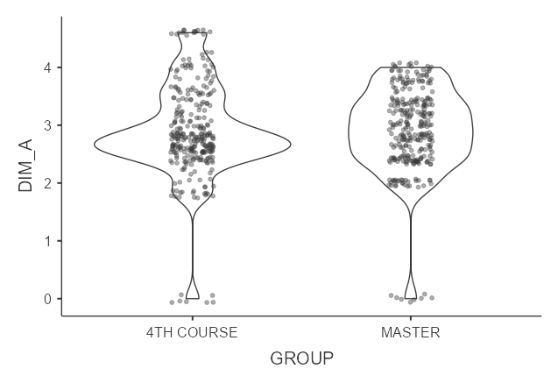
\includegraphics[width=\textwidth]{fig1.png}
\source{Captura de pantalla del libro de \textcite[p. 96]{kalantzis2019} \emph{Las alfabetizaciones múltiples, teoría y práctica}.}
\end{minipage}
\end{figure}
	
Este enfoque fue presentado en sesiones teóricas a los futuros docentes
y discutido dentro de las clases programadas en la asignatura para su
posible inclusión en los proyectos de innovación que serían realizados
en su práctica profesional. Además, se motivó el diseño de experiencias
de mediación de la literatura que incluyeran las prácticas de
literacidad y literacidad digital de sus estudiantes.

A partir de la consideración de ambos enfoques, se elaboraron unos
criterios (\Cref{tab-03}) que, finalmente, apoyaron la valoración de la
experiencia y del despliegue de las literacidades digitales de un grupo
de futuros profesores de lengua y literatura en sus portafolios.

\begin{table}[!htpb]
\centering
\begin{threeparttable}
\caption{Descripción de los criterios utilizados en la valoración de los portafolios.}
\label{tab-03}
\begin{tabular}{lp{5cm}p{5cm}}
\toprule
	& Literacidades digitales & Mediación desde las multiliteracidades. \\
\midrule
Desarrollo cognitivo & Despliegue de literacidades digitales desde la visión de la cultura de la web/ motivación del uso. & Análisis y/o interpretación. Tipo de lecturas escogidas. Encuadre: experimentar desde lo conocido o lo nuevo. \\
Significado & Uso de la plataforma Sites. Multimodalidad. Hipertextualidad/uso de enlaces. & Agencia del estudiantado (herramientas de creación). Aplicar creativamente y/o apropiadamente. \\
Autenticidad y acceso & Selección de herramientas y tipo de uso. Presentación desde la identidad digital. & Mediación a partir de alguno de los procesos de conocimiento de las multiliteracidades. \\
\bottomrule	
\end{tabular}
\source{Elaboración propia.}
\end{threeparttable}
\end{table}

\subsection{Valoración de las literacidades digitales y mediación de la literatura}\label{sub-sec-valoracióndelas}
	A continuación, se expondrá la valoración de los portafolios desde las
	dimensiones de las literacidades digitales y el enfoque de la pedagogía
	de las multiliteracidades, por medio de los criterios expuestos en el
	apartado anterior.

\subsubsection{Desarrollo cognitivo}\label{sub-sub-sub-sec-desarrollo}

Esta dimensión se valoró desde la visión de la cultura de internet y las
redes sociales. La mediación desde las multiliteracidades se apreció
desde el encuadre y el tipo de análisis propuesto.

Desde la perspectiva de las literacidades digitales, se pudo observar en
algunos portafolios el uso de memes y el lenguaje de las redes sociales
(\Cref{fig-02}). Sin embargo, dicho uso no fue común en la totalidad de los
portafolios valorados, ya que en varios de ellos se observó la presencia
de prácticas de literacidad que pertenecen al ámbito académico, cuyo
énfasis está en el código escrito. No obstante, dicho código estaba
acompañado de vídeos, audios e imágenes.

\begin{figure}[htpb]
\centering
\begin{minipage}{.7\textwidth}
\caption{Uso de memes vinculados con la cultura de internet y que fueron utilizados en la reflexión realizada por el docente en formación en su portafolio.}
\label{fig-02}
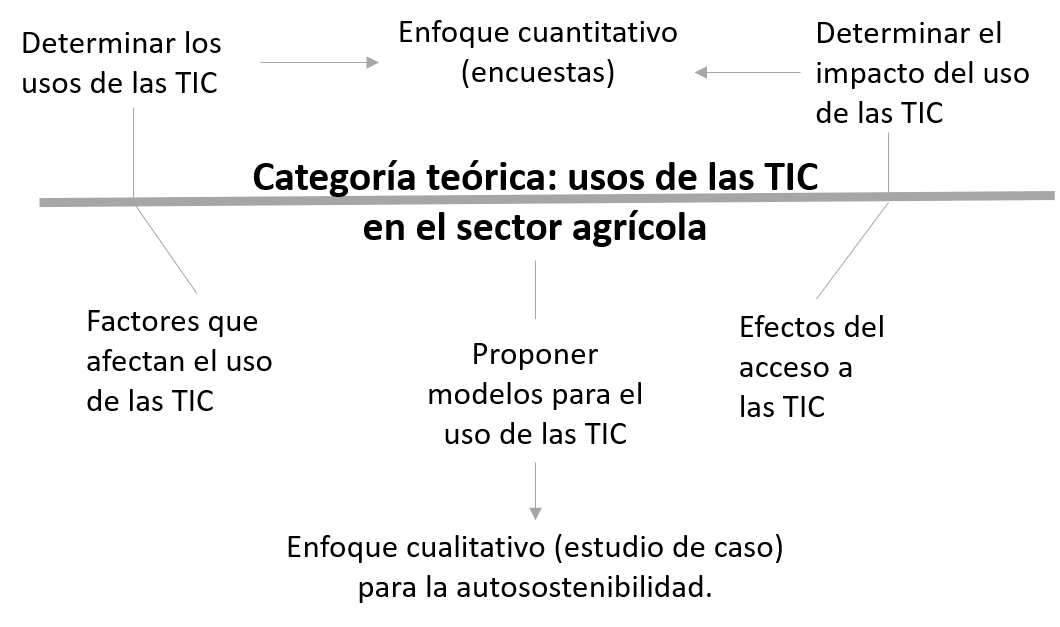
\includegraphics[width=\textwidth]{fig2.png}
\source{Captura de pantalla del portafolio ``\href{https://sites.google.com/view/portafolio-sergio-gonzlez}{Practicando -ando}''.}
\end{minipage}
\end{figure}

En algunos portafolios se puede visualizar que los futuros profesores
utilizaron la gamificación para explicar sus trayectorias o para
introducir al lector en un ámbito reflexivo nuevo. Esto fue uno de los
aspectos que sobresalió dentro de los portafolios visualizados. Sin
embargo, en rasgos generales, se puede señalar que prefieren utilizar la
interfaz proporcionada por Sites por defecto, sin alterarla demasiado.

Dentro de esta dimensión, lo que refiere a las experiencias de mediación
relatadas, en la mayoría de los portafolios se pudo observar que se
realizaban desde el proceso de conocimiento de experimentar lo nuevo, ya
que eran los profesores en formación quienes presentaban un recurso que
pudiera ser del interés de sus estudiantes y que, luego de su análisis y
discusión, era utilizado para presentar el texto literario que sería
interpretado, como se puede apreciar en la \Cref{tab-04}.

\begin{table}[!htpb]
\centering
\begin{threeparttable}
\caption{Ejemplo de recursos utilizados dentro del proceso ``experimentar lo nuevo'' conectado con el análisis e interpretación de obras literarias.}
\label{tab-04}
\begin{tabular}{llp{3cm}p{3cm}p{3cm}}
\toprule
Portafolio & OA & Recurso & Proceso de conocimiento & Obra literaria \\
\midrule
Practicando-ando & OA8 & Vídeo
\href{https://youtu.be/DUGtyj5QlEM?si=_KwsI8ND0PrJCqJ3}{``Dos oruguitas}'' (Sebastián Yatra). & Experimentar lo nuevo. Conceptualizar desde la teoría. & Poema de Emily Dickinson. \\
Portafolio NL & OA4 & \href{https://sites.google.com/view/portafolio-nicolas-lagos/repertorio-de-muestras/segunda-muestra-desafíos}{Canción ``The book of you and I}'' (Alec Benjamin). & Experimentar lo nuevo. Analizar funcional y críticamente. & ``La esperanza es esa cosa con plumas'' Emily Dickinson; ``Espejo'' Silvia Plath. \\
Portaflores & OA2 & Corto animado: ``\href{https://youtu.be/to8yh83jlXg?si=rPhsC7o_mtj8rDCp}{The last Bastion}'' (Overwatch). Microcuento \href{https://santiagoen100palabras.cl/en-vitrina/}{``En vitrina''} (Valentina Sandoval). & Experimentar lo conocido/lo nuevo. & Tema del viaje. \\ 
\bottomrule
\end{tabular}
\end{threeparttable}
\end{table}
	
\subsubsection{Significado}\label{sub-sub-sec-significado}

Esta dimensión se valoró a través del uso que realizaron los docentes en
formación de la plataforma Sites, la idea de diseño desde la
multimodalidad y el hipertexto desde la creación de itinerarios libres.
A su vez, se procuró observar el desarrollo de la agencia del
estudiantado a través del proceso de conocimiento de aplicar de forma
apropiada o creativa, u otro vinculado a las multiliteracidades, en las
experiencias de mediación presentadas según el OA escogido.

Se puede señalar que, en forma general, en los portafolios observados se
utiliza el hipertexto como una forma de expresión y creación dentro de
la plataforma Sites. Una de las plataformas que permitió estos
itinerarios fue Genially, ya que en algunos portafolios fue la base de
los itinerarios propuestos (\Cref{fig-03}) plataforma permite una
interacción y navegación entre diversos hipervínculos. Otra herramienta
que permitió la creación de itinerarios, fue Slides de Google, ya que la
misma plataforma Sites facilita su inserción.

\begin{figure}[htpb]
\centering
\begin{minipage}{.7\textwidth}
\caption{ejemplo de un itinerario propuesto a través de la herramienta Genially.}
\label{fig-03}
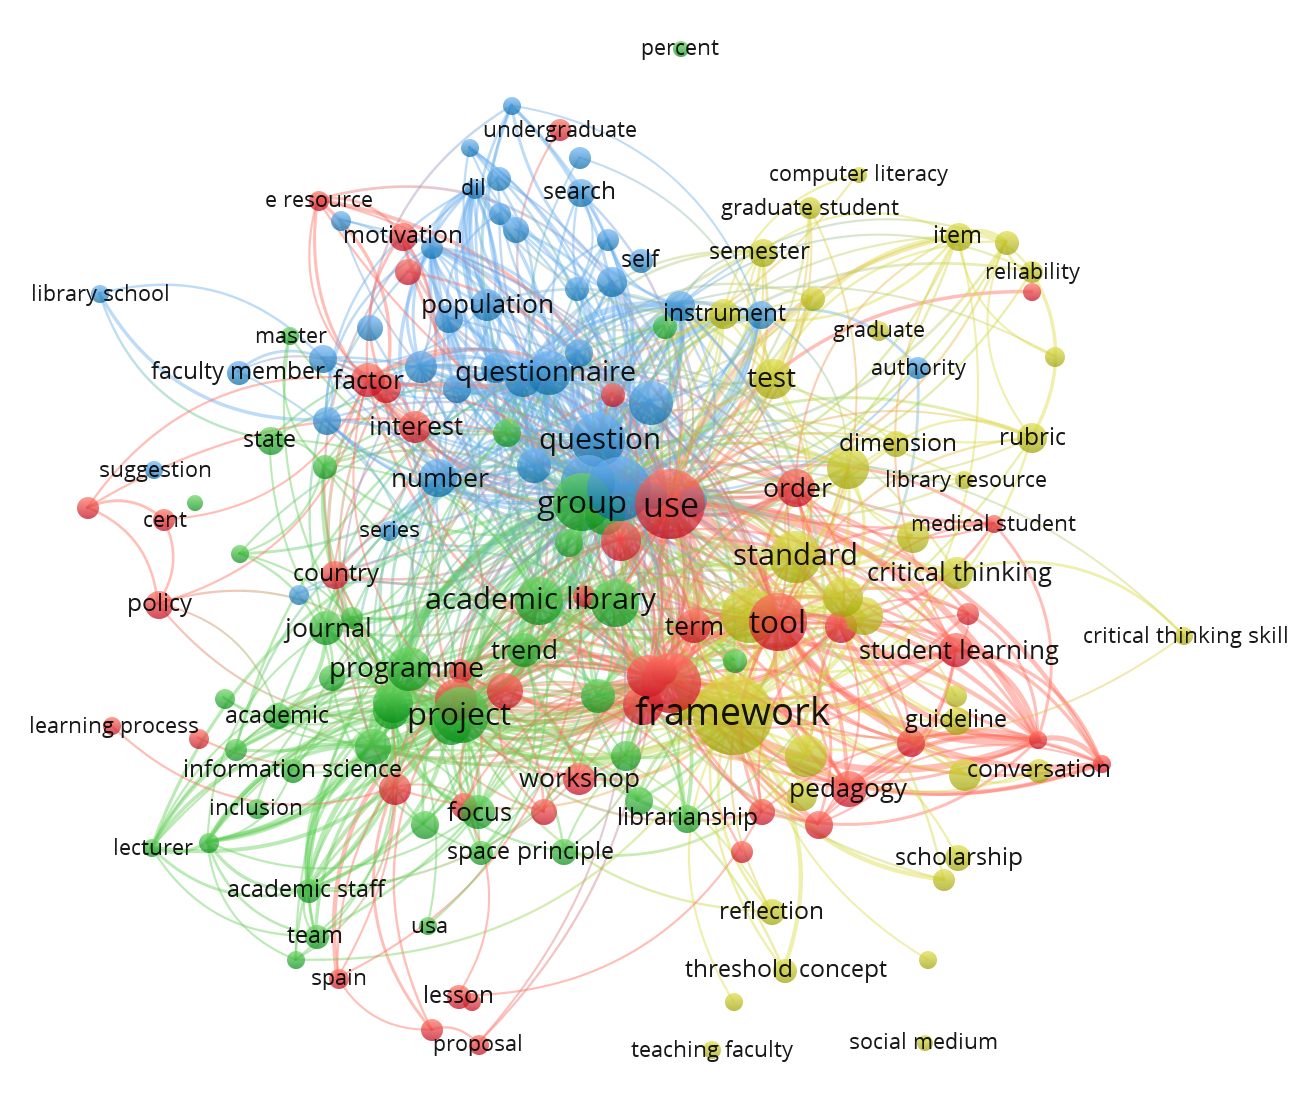
\includegraphics[width=\textwidth]{fig3}
\source{Captura de pantalla del portafolio ``\href{https://sites.google.com/view/rosaerium-portaflores/has-llegado-a-tu-nuevo-destino/misión-2-hay-un-extraño-no-no-soy-yo}{Portaflores}''.}
\end{minipage}
\end{figure}


La combinación de recursos que permite la plataforma Sites, facilitó a
los futuros docentes diseñar su portafolio como un texto multimodal e
hipertextual y, por tanto, que cada uno de los portafolios lograra un
diseño particular y único.

El uso de diferentes recursos dentro de los portafolios digitales se
enlaza de alguna manera con los procesos de mediación de la lectura
presentados. Esto pudo observarse a través de la aplicación apropiada o
creativa según el proceso de conocimiento de las multiliteracidades
escogido. Algunas de las actividades realizadas bajo dicho proceso,
fueron concebidas para que los estudiantes de aula pudieran comprender
los conceptos que les servirían para analizar textos literarios de
acuerdo con el OA de la secuencia planificada (\Cref{fig-04}). Con este fin,
los futuros docentes recurrieron al uso de recursos digitales conocidos
y utilizados en sus portafolios.

\begin{figure}[htpb]
\centering
\begin{minipage}{.7\textwidth}
\caption{Ejemplo de actividad de mediación de acuerdo al OA 4, la creación de un diccionario simbólico a través de la herramienta Padlet.}
\label{fig-04}
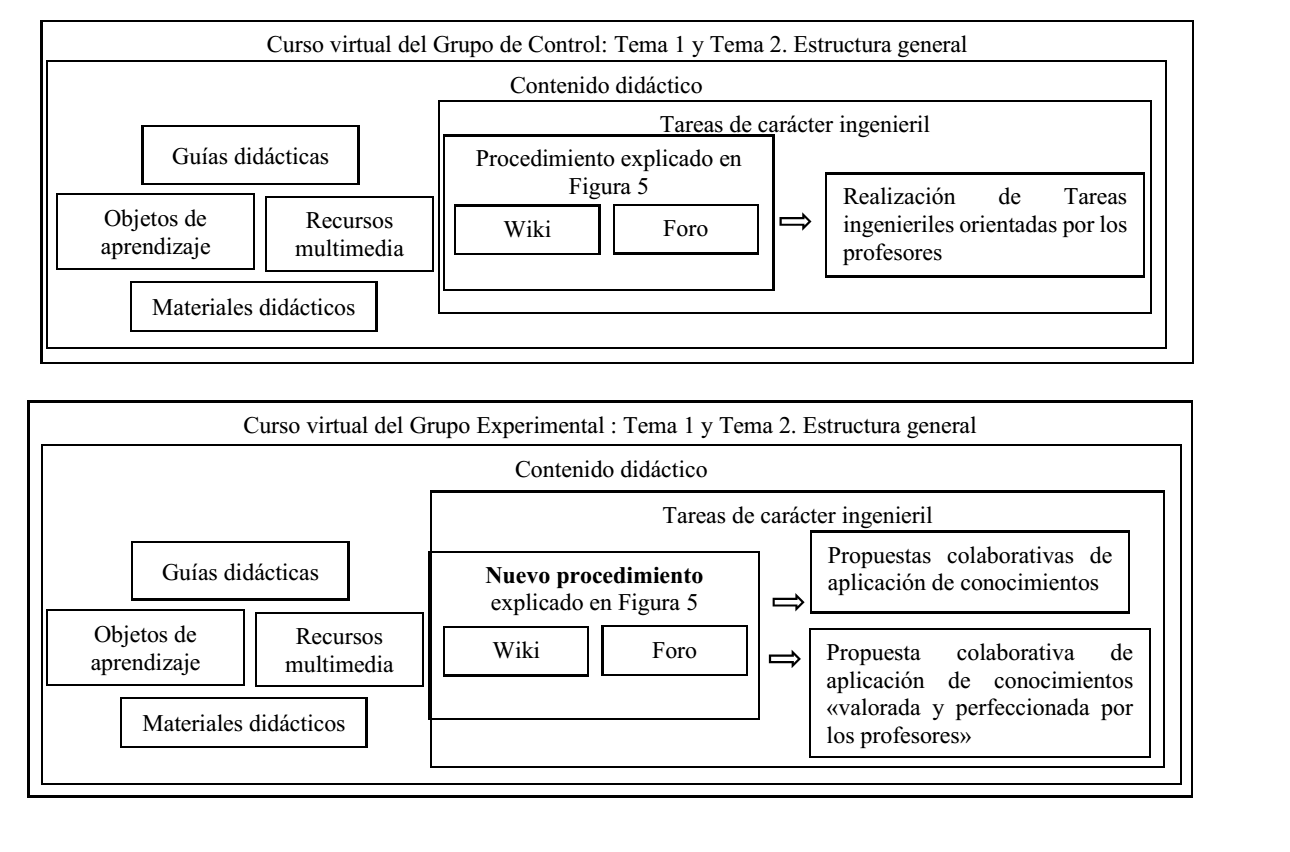
\includegraphics[width=\textwidth]{fig4.png}
\source{Captura de pantalla del portafolio ``\href{https://sites.google.com/view/portafolio-nicolas-lagos/repertorio-de-muestras/segunda-muestra-desafíos}{Portafolio NL}''.}
\end{minipage}
\end{figure}

\subsubsection{Autenticidad y acceso}\label{sub-sub-sec-autenticidad}

En esta dimensión se valoró a los portafolios desde la selección de
herramientas digitales y su uso. Desde la experiencia de mediación,
interesaba observar la proyección de los procesos de conocimiento de las
multiliteracidades narrados en los portafolios.

En todos los portafolios, la herramienta más utilizada fue Genially, ya
que es una plataforma que permite la interactividad y la creación de
textos multimodales. Otras de las herramientas utilizadas fueron Padlet
y YouTube.

Cabe precisar que el diseño de la plataforma Sites fue utilizado por
defecto en el diseño de los portafolios, sobre todo en lo que respecta
al uso de pestañas como hipervínculos. En esto último, también fue muy
utilizada la plataforma Slides y Docs de Google, ya que la plataforma
facilitaba la inserción de estos recursos.

En el caso de YouTube, este fue empleado para exponer vídeos generados
por Zoom, semejante, en este sentido, a una exposición oral. También
dicha plataforma fue utilizada en algunos casos como \emph{podcast}
(\Cref{fig-05}) y, por tanto, sin el énfasis divulgativo y social inherente a
esta plataforma.

\begin{figure}[htpb]
\centering
\begin{minipage}{\textwidth}
\caption{Ejemplo de uso de la plataforma YouTube como \emph{podcast.}}
\label{fig-05}
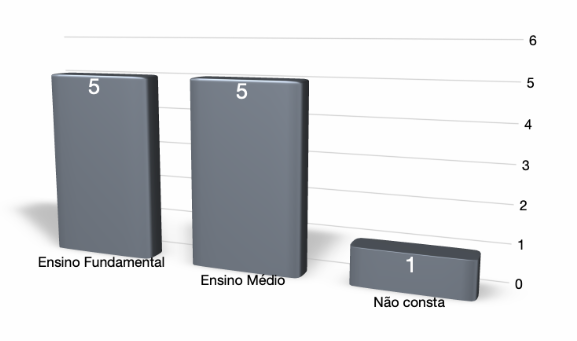
\includegraphics[width=\textwidth]{fig5}
\source{Captura de pantalla del portafolio ``\href{https://sites.google.com/view/portafolio-pdye/introducción}{Portafolio Pdye}''.}
\end{minipage}
\end{figure}

Sobre esto último, es necesario mencionar que, en la valoración de los
portafolios, se pudo distinguir que hay un predominio de prácticas de
literacidad académicas, ya que el código escrito estaba presente en la
mayoría de las presentaciones realizadas (con Slides y Genially) y en el
contenido de las pestañas de los portafolios.

Lo anterior se condice, en cierto modo, con el desarrollo de las
experiencias de mediación, ya que, dentro de los procesos de
conocimiento de las multiliteracidades, hay un predominio de la
experimentación desde lo nuevo, que da paso a estrategias tradicionales
de lectura desarrolladas a través de procesos psico-cognitivos. Los
espacios de discusión y análisis de los textos literarios se dan dentro
de los procesos de experimentación o análisis crítico. Los procesos de
conceptualización son los menos abordados.

\section{Reflexiones finales y conclusiones}\label{sec-reflexionesfinalesyconclusiones}

La experiencia desarrollada en este artículo tenía como objetivo
responder a preguntas vinculadas con los desafíos que tiene la lectura
en la actualidad. Dichos desafíos están implicados con las literacidades
digitales de los docentes en formación de lengua y literatura. Para
ello, interesaba observar de qué manera interactuaban sus literacidades
con el diseño de proyectos que integran la lectura literaria a través de
la pedagogía de las multiliteracidades.

Uno de los primeros objetivos de la experiencia pretendía que los
profesores en formación desarrollaran sus literacidades digitales en los
portafolios reflexivos digitales. En relación con este objetivo, si bien
la muestra es muy acotada, es significativa en cuanto a que proporciona
una idea del tipo de literacidades digitales que posee un grupo de
estudiantes de pedagogía en un contexto académico y en el que deben
reflexionar sobre sus experiencias de mediación de la literatura.

Dentro de las dimensiones de las literacidades digitales se puede
señalar que, en estos futuros docentes, el ámbito digital es natural
dentro de sus prácticas, considerando, además su rango de edad. Esto se
demuestra por el despliegue de herramientas utilizadas en la plataforma
Sites y la idea de diseño de cada uno de los portafolios. En ellos se
pudo ver prácticas próximas al lenguaje de las redes sociales y
culturales como el uso de memes, la gamificación e itinerarios
proporcionados por las diversas plataformas utilizadas, que podría ser
una aproximación a una competencia digital pedagógica como la han
propuesto Silva et al. (2019), Sandoval Rubilar; Rodríguez Alveal;
Maldonado Fuentes (2017) y Ayala (2015), aunque de manera indirecta, ya
que el despliegue de literacidades digitales podría aportar algunas
luces a la problemática sobre la competencia digital en la formación
inicial docente.

El diseño de los portafolios y los itinerarios propuestos pueden
entenderse dentro de la idea de multimodalidad, en el sentido de que,
tanto en los portafolios como en las experiencias de mediación, se pudo
observar rediseños que obedecían a un modo particular de entender la
experiencia de creación de los portafolios y la aproximación de textos
literarios en el aula. Esto último se asemeja en parte a lo señalado por
Fernandes (2018) en lo que refiere a la reconstrucción más amplia de los
textos, que, en estos casos, fue a través de los productos culturales
desarrollados y el uso que se dio a las plataformas digitales.

Sobre esto último, llamó la atención el uso que se dio a la plataforma
YouTube en varios de los portafolios observados, pues dicha herramienta
fue utilizada para incrustar vídeos realizados a través de la plataforma
Zoom, con un claro propósito expositivo. Esto último podría ser
consecuencia de la digitalización de la enseñanza en la pandemia, ya que
dicha plataforma se incorporó masivamente dentro de la docencia en la
universidad y, por tanto, formó parte de las prácticas digitales de ese
periodo.

El uso de la plataforma YouTube de esta manera, invita a reflexionar
sobre el conocimiento ético de su uso, así como del tema de la
privacidad en el ciberespacio. Se señala lo anterior, porque en la
mayoría de los vídeos compartidos a través de esta plataforma, están en
modalidad pública, siendo que existe la opción de ocultarlos o hacerlos
privados.

En la valoración de los portafolios se pudo observar que las
herramientas y plataformas incorporadas por los futuros docentes en sus
portafolios, tienen una finalidad predominantemente formativa. Es el
caso de Genially, Padlet, Slide y Docs de Google, que son herramientas
ampliamente utilizadas en el ámbito educativo y, por tanto, su uso
informa de las literacidades digitales de futuros docentes dentro del
ámbito académico. No obstante, lo anterior, dentro de las experiencias
de mediación se apreció el uso de YouTube y Padlet, pero no de Genially,
debido, probablemente, al nivel de conexión a internet que se necesita
para su funcionamiento y que, en escuelas vulnerables, es un recurso que
escasea o es débil.

Esto último pudo haber repercutido en el desarrollo de las experiencias,
ya que muchas de ellas utilizaron recursos analógicos más que digitales,
que afectó la agencia del estudiantado. Probablemente, la escasez de
dispositivos interactivos dificulta la diversificación de estrategias,
coincidiendo con el análisis de Ramada Prieto y Turrión Penelas (2019) y
lo señalado por Ryan (2004). Pese a lo anterior, la incorporación de la
cultura de internet en las experiencias pudo haber impactado el
desarrollo de las estrategias de mediación.

Se señala lo anterior, ya que se pudo apreciar que la incorporación de
los procesos de conocimiento, especialmente los procesos de
experimentación desde lo nuevo o lo conocido y el análisis crítico, dio
un énfasis menos tradicional al proceso de mediación literaria. Esto se
puede visualizar a partir de las actividades desarrolladas por los
profesores en formación, ya que, en su mayoría, estas se llevaban a cabo
a partir de artefactos y manifestaciones culturales-digitales conocidas
tanto por ellos como por sus estudiantes, y no necesariamente desde el
texto literario en sí. Esto último concuerda con la idea de sinestesia
propuesta por Kalantzis, Cope y Zapata (2019), ya que para interpretar
un texto literario, los profesores presentaban a sus estudiantes una
aproximación a los textos desde distintas modalidades que les
posibilitara realizar una interpretación estética o crítica.

En las estrategias de mediación se puede observar que se discutían y
analizaban las manifestaciones culturales conocidas a partir de
temáticas vinculas a los OA trabajados. A partir de dicha discusión, se
presentaba el texto literario, el cual, la mayoría de las veces se
analizaba a partir de estrategias de lectura convencionales. Sin
embargo, al llevar a cabo los procesos de conocimiento de las
multiliteracidades, los docentes en formación generaron instancias en
las que sus estudiantes pudieron aplicar de forma apropiada o creativa.
En este sentido, la creación se enfoca desde los productos culturales y
la interpretación de los textos literarios considera elementos más
emocionales y, en algunos casos, más estructurales, que puede deberse al
contexto de retorno de la pandemia y de los OA seleccionados para el
proyecto. Se podría decir que las experiencias se aproximan, levemente,
a lo señalado por Meneses, Maturana y Báez (2024), lo que indica que es
necesario seguir trabajando desde este enfoque.

Se puede señalar, por tanto, que la mediación de la literatura a través
de la pedagogía de las multiliteracidades en los portafolios observados,
integra parte de las literacidades digitales de los profesores en
formación, ya que el modo de aproximar la lectura literaria en los
discentes está matizado por la experiencia digital, que les permite
tener una visión diferente sobre la mediación de lectura literaria en el
aula. Esto último, se condice con las experiencias llevadas a cabo por
Godoy (2023) y Cabré Rocafort (2021) respecto al enfoque de las
multiliteracidades en la formación inicial docente y la mediación
lectora.

Respecto a las escuelas que tienen un alto índice de vulnerabilidad, se
puede decir que el uso de ciertas herramientas y plataformas conocidas
por este grupo de profesores en formación, facilitó la lectura de textos
más complejos en los estudiantes y ayudó a que estos realizaran una
interpretación o creación a partir del desarrollo de su punto de vista
sobre dichos textos; por lo tanto, el enfoque de las multiliteracidades
podría ser una oportunidad para avanzar en la disminución de la
desigualdad que presentan estas escuelas.

Como conclusión, se puede señalar que es necesario crear instancias
formativas que permitan a los futuros docentes desplegar sus
literacidades digitales y que estas puedan ser concientizadas por ellos,
de modo que puedan integrarlas en los procesos de mediación de la
literatura. Al respecto, la experiencia relatada quiso ser un aporte a
la comprensión de nuevas formas de mediación de la literatura que
integran prácticas ligadas a una visión del uso digital, a través del
enfoque pedagógico de las multiliteracidades.

Las limitaciones de la experiencia son variadas, está la cantidad de
portafolios valorados, el contexto de retorno a la pandemia y la
necesidad de datos más empíricos que pudo haber afectado la valoración.
También dentro de las limitaciones podemos señalar el acceso a la
recepción de los estudiantes de aula sobre esta experiencia, que puede
pensarse como futuras investigaciones sobre este tema.

Pese a lo anterior, se piensa que la descripción de esta experiencia
puede ser un insumo interesante para dar a conocer un enfoque que se
está trabajando dentro de la formación inicial docente de una
universidad pública en Chile. También la valoración de estos
portafolios, pretende ser una contribución a estudios sobre la pedagogía
de las multiliteracidades que abordan experiencias de mediación de la
literatura.

La experiencia descrita, además, es una invitación a profundizar en las
prácticas de literacidad digital de futuros docentes de lengua y
literatura para reflexionar sobre el impacto en su ejercicio docente, su
concepción de la literatura y la mediación en las aulas, que implicaría
un estudio más profundo que permita dilucidar conclusiones más robustas
sobre estos temas, que adquieren relevancia dentro del contexto
desafiante e incierto que deben enfrentar las escuelas en la actualidad.

 \section{Financiación}
Este estudio fue apoyado por la Vicerrectoría de Investigación y Desarrollo (VID) de la Universidad de Chile, a través del concurso “Ayuda de Viajes para Potenciar la Productividad Académica VID, 2024” (AYV077/01-23).


\printbibliography \label{sec-bib}

\appendix
\section{Sites de la asignatura. Exposición de la experiencia}

\url{https://sites.google.com/uchile.cl/proyectosdyeinnovadores/inicio?authuser=0}
 
\section{Objetivos de aprendizaje de las experiencias}\label{sec-annex}

\begin{small}
\begin{longtable}{p{2cm}cp{7cm}}
\caption{Objetivos de aprendizaje de las experiencias}
\label{annex-tab01}
\\
\toprule
OA/unidad trabajada & Nivel & Descripción del objetivo\\
\midrule
OA8/El amor y la lírica & 8º básico & Formular una interpretación de los textos literarios leídos o vistos, que sea coherente con su análisis, considerando:
\begin{itemize}
\item Su experiencia personal y sus conocimientos.
\item Un dilema presentado en el texto y su postura personal acerca del mismo.
\item La relación de la obra con la visión de mundo y el contexto histórico en el que se ambienta y/o en el que fue creada.
\end{itemize} \\

OA2 & 3º medio & Reflexionar sobre el efecto estético de las obras leídas, evaluando: 
\begin{itemize}
\item Cómo la obra dialoga con las experiencias personales del lector y sus puntos de vista sobre diversas problemáticas del ser humano (afectos, dilemas éticos, conflictos, etc.).
\item Cómo los recursos y técnicas literarias de la obra inciden en el efecto estético producido.
\end{itemize}
\\
OA1 & 3º medio & Formular interpretaciones surgidas de sus análisis literarios, considerando:
\begin{itemize}
\item La contribución de los recursos literarios (narrador, personajes, tópicos literarios, características del lenguaje, figuras literarias, etc.) en la construcción del sentido de la obra.
\item Las relaciones intertextuales que se establecen con otras obras leídas y con otros referentes de la cultura y del arte.
\end{itemize}
\\
OA4 & 2º medio & Analizar los poemas leídos para enriquecer su comprensión, considerando, cuando sea pertinente:
\begin{itemize}
\item Los símbolos presentes en el texto y su relación con la totalidad del poema.
\item La actitud del hablante hacia el tema que aborda.
\item El significado o el efecto que produce el uso de lenguaje figurado en el poema.
\item El efecto que tiene el uso de repeticiones (de estructuras, sonidos, palabras o ideas) en el poema.
\item La relación que hay entre un fragmento y el total del poema.
\item Relaciones intertextuales con otras obras.
\item Las características del soneto.
\end{itemize}
 \\
OA2 & 2º medio & Reflexionar sobre las diferentes dimensiones de la experiencia humana, propia y ajena, a partir de la lectura de obras literarias y otros textos que forman parte de nuestras herencias culturales, abordando los temas estipulados para el curso y las obras sugeridas para cada uno. \\
OA3/Literatura de terror y ciencia ficción & 8º básico & Analizar las narraciones leídas para enriquecer su comprensión, considerando, cuando sea pertinente:
\begin{itemize}
\item El o los conflictos de la historia.
\item Los personajes, su evolución en el relato y su relación con otros personajes.
\item La relación de un fragmento de la obra con el total.
\item El narrador, distinguiéndolo del autor.
\item Personajes tipo (por ejemplo, el pícaro, el avaro, el seductor, la madrastra, etc.), símbolos y tópicos literarios presentes en el texto.
\item Los prejuicios, estereotipos y creencias presentes en el relato y su conexión con el mundo actual.
\item La disposición temporal de los hechos, con atención a los recursos léxicos y gramaticales empleados para expresarla.
\item Elementos en común con otros textos leídos en el año.
\end{itemize}
\\
\bottomrule
\source{Elaboración propia.}
\end{longtable}
\end{small}

\end{document}
